\documentclass[11pt]{article}

\usepackage[T1]{fontenc}
\usepackage{tgpagella}
\usepackage[scale=0.92]{tgheros}
\usepackage[scale=0.88]{tgcursor}
\usepackage{amsmath}
\usepackage[italic,defaultmathsizes]{mathastext}

\usepackage[a4paper, margin=16.5mm, top=15mm, bottom=16mm, headheight=15pt]{geometry}
\usepackage{microtype}
\usepackage{parskip}
\usepackage[table]{xcolor}
\usepackage{tikz}
\usepackage{booktabs}
\usepackage{tabularx}
\usepackage{array}
\usepackage{enumitem}
\usepackage{titlesec}
\usepackage{fancyhdr}
\usepackage[most]{tcolorbox}
\usepackage{float}
\usepackage{needspace}
\usepackage{hyperref}
\urlstyle{same}
\def\UrlBreaks{\do\/\do\-}

\definecolor{ebdink}{HTML}{1C2834}
\definecolor{ebdgreen}{HTML}{0F6E56}
\definecolor{ebdgreenpale}{HTML}{E6F4EF}
\definecolor{ebblue}{HTML}{1E4D7B}
\definecolor{ebbluepale}{HTML}{E7F0F8}
\definecolor{ebamber}{HTML}{8A4B08}
\definecolor{ebamberpale}{HTML}{FBF4E6}
\definecolor{ebdmuted}{HTML}{5C6B7A}
\definecolor{ebdtrack}{HTML}{E3E8ED}
\definecolor{ebdrow}{HTML}{F6F8FA}
\definecolor{ebdwomen}{HTML}{0F6E56}
\definecolor{ebdmen}{HTML}{C56A12}

\hypersetup{
  colorlinks = true,
  linkcolor = ebblue,
  urlcolor = ebdgreen,
  pdftitle = {Where the bias sits},
  pdfauthor = {EBD-AI},
  pdfsubject = {Fuzzy rules, explainable-by-design models, and bias demos 9, 10 and 11},
}

\setlist[itemize]{itemsep=0.28em, topsep=0.35em, leftmargin=1.25em}
\setlist[enumerate]{itemsep=0.28em, topsep=0.35em, leftmargin=1.35em}
\newcolumntype{Y}{>{\raggedright\arraybackslash}X}
\renewcommand{\arraystretch}{1.18}

\titleformat{\section}
  {\sffamily\large\bfseries\color{ebdink}}
  {\thesection}{0.55em}{}
  [\vspace{-0.55em}{\color{ebdgreen}\titlerule[1.15pt]}\vspace{0.15em}]
\titlespacing*{\section}{0pt}{1.15em}{0.55em}
\titleformat{\subsection}
  {\sffamily\bfseries\color{ebblue}}
  {\thesubsection}{0.5em}{}
\titlespacing*{\subsection}{0pt}{0.85em}{0.3em}

\pagestyle{fancy}
\fancyhf{}
\fancyhead[L]{\sffamily\small\color{ebdmuted}EBD-AI}
\fancyhead[R]{\sffamily\small\color{ebdmuted}Bias demos 9--11}
\fancyfoot[L]{\sffamily\small\color{ebdmuted}Where the bias sits}
\fancyfoot[R]{\sffamily\small\color{ebdmuted}\thepage}
\renewcommand{\headrulewidth}{0pt}
\renewcommand{\footrulewidth}{0pt}
\fancyheadoffset{0pt}

\tcbset{
  enhanced,
  breakable,
  boxrule = 0pt,
  arc = 2.5pt,
  boxsep = 1.5pt,
  left = 8pt,
  right = 8pt,
  top = 5pt,
  bottom = 5pt,
  before skip = 8pt,
  after skip = 8pt,
}

\newtcolorbox{lesson}{
  colback = ebdgreenpale,
  colframe = ebdgreenpale,
  borderline west = {3pt}{0pt}{ebdgreen},
}
\newtcolorbox{idea}{
  colback = ebbluepale,
  colframe = ebbluepale,
  borderline west = {3pt}{0pt}{ebblue},
}
\newtcolorbox{careful}{
  colback = ebamberpale,
  colframe = ebamberpale,
  borderline west = {3pt}{0pt}{ebamber},
}

\newcommand{\fn}[1]{\texttt{\small #1}}
\newcommand{\track}[2]{%
  \begin{tikzpicture}[baseline=-0.15ex]
    \fill[ebdtrack] (0,0) rectangle (5.55,0.20);
    \fill[#2] (0,0) rectangle ({5.55*(#1)},0.20);
  \end{tikzpicture}%
}
\newcommand{\pct}[1]{\mbox{#1\%}}

\begin{document}
\color{ebdink}
\raggedbottom
\thispagestyle{fancy}

\begin{tcolorbox}[
  colback=ebdink, colframe=ebdink, arc=3pt,
  left=12pt, right=12pt, top=9pt, bottom=9pt,
  before skip=0pt, after skip=8pt,
]
{\color{white}\sffamily\bfseries\fontsize{21}{25}\selectfont Where the bias sits\par}
\vspace{3pt}
{\color{white!88}\sffamily Fuzzy rules, explainable-by-design models,\par and the Titanic, heart-failure, and loan notebooks\par}
\end{tcolorbox}

\noindent
The guide has two parts. The first is the foundation: what it means for a model to be explainable by design, why the European rules ask for an explanation a person can read, and how a fuzzy rule-based classifier produces that explanation. The second part reads the three bias notebooks that use this classifier. The rule learner is \fn{ex\_fuzzy}. The bias measurements live in \fn{ebdai}. The tables come from the WorkshopIgualdad2025 materials shipped inside the package.

% ---------------------------------------------------------------------
\section{Explainable by design}
\label{sec:ebd}

BDI is the Explainable By Design AI toolbox. The phrase is the definition. A model is explainable by design when the thing you trained is already a description a person can read. The decision and the explanation are the same object.

In these notebooks that object is a short list of if--then rules. Ask why one passenger was predicted to survive, and the answer is a sentence you can point at, plus a number saying how strongly the sentence matched that passenger. \fn{explainable\_predict} returns that explanation directly: the predicted class, the index of the winning rule, and the match.

\begin{idea}
\textbf{Two ways to explain a model.} A post-hoc explanation trains an opaque model, such as a neural net or a large ensemble, and afterwards builds a second story about it: a saliency map, a list of feature scores, or a simpler model fitted to copy it. That second story can be useful, and it can disagree with the model that decided. An explainable-by-design model keeps the decision procedure in a form you audit directly. Here, you audit the sentences that fire.
\end{idea}

That audit can see three things a block of weights does not show as text.

\begin{enumerate}
  \item \textbf{What the model is allowed to say.} Each rule names columns in ordinary words. When sex is used, the word sex is in the sentence.
  \item \textbf{Who each sentence decides for.} The winning-rule count says how often that sentence is the one that fires, inside each group.
  \item \textbf{What the training score rewarded.} Demo 11 changes the score. The model remains a list of rules, so you can see whether the new score changed the sentences, the rates, or both.
\end{enumerate}

\begin{careful}
\textbf{Readable describes the model. Fair describes the decisions.} A rule that says ``sex is female'' is easy to audit, and it can still be a biased rule. A rule that never writes the word sex can still track sex through fare, marriage, or income. Explainable by design makes those checks possible. The checks are the measurements in Section~\ref{sec:measure} and the three demos that follow.
\end{careful}

\fn{ex\_fuzzy} is the fuzzy-rule family, the first family shipped in the toolbox. \fn{ebdai} is where further explainable-by-design tools live. In these notebooks that means the bias measurements and the two altered training scores in the loan demo. The same design idea also covers other readable families in the library, including fuzzy rule trees and conformal prediction sets. Demos 9--11 use the fuzzy classifier only.

% ---------------------------------------------------------------------
\section{Why the rules ask for an explanation}
\label{sec:law}

Explainability matters here because a person on the receiving end of a serious decision, and the person asked to oversee the system, both have to be able to see how that outcome was produced. In September 2026 the European rules already require that for many automated decisions about people. A further set of duties, written specifically for high-risk AI, is on the statute book with later start dates. This section is a map of those duties. It is not legal advice, and a classroom notebook is not a system placed on the market.

\subsection{The explanation already owed to one person}

Where a decision is based solely on automated processing of personal data and has a legal effect, or a similarly serious effect, the GDPR restricts it and, where it is allowed, requires safeguards: a human can intervene, the person can state their view, and the person can contest the decision (Article~22). Contesting a decision depends on knowing the reason.

Articles~13(2)(f), 14(2)(g) and~15(1)(h) require ``meaningful information about the logic involved''. On 27~February 2025, in \emph{CK v Dun \& Bradstreet Austria} (C-203/22), a case about an automated credit assessment, the Court of Justice said what that phrase demands. The controller must describe the procedure and principles actually applied, so that the person can understand which of their data were used and how. The explanation has to be concise and intelligible. Communicating the algorithm, or a long trace of every internal step, does not meet that standard. A trade secret is not a reason to refuse any explanation.

A winning fuzzy rule is the shape of answer that standard describes. ``This application was refused because the rule that fired was: credit history is poor, and income is Low.'' The person can see the data that mattered and the principle that used them. A file of network weights does not do that work.

\subsection{High-risk AI, on a published timetable}

Regulation~(EU)~2024/1689, the AI Act, entered into force on 1~August 2024. Its duties start in stages. Regulation~(EU)~2026/1744, in force from 27~July 2026, moved only the high-risk timetable. It left the rest of the Act in place.

\begin{table}[H]
\centering
\small
\begin{tabularx}{\textwidth}{@{}l Y@{}}
\toprule
From & What applies \\
\midrule
2 February 2025 & Prohibited practices, and the duty to ensure a sufficient level of AI literacy. \\
\rowcolor{ebdrow}
2 August 2025 & Duties for general-purpose AI models. \\
2 August 2026 & The Act's remaining provisions, apart from the high-risk duties dated below. Article~50 applies: people are told when they are interacting with an AI system, and certain synthetic content is labelled. \\
\rowcolor{ebdrow}
2 December 2027 & High-risk duties for stand-alone systems in Annex~III. Creditworthiness scoring of a natural person is one of those uses. \\
2 August 2028 & High-risk duties for AI that is, or sits inside, a regulated product. Many medical devices fall on this date. \\
\bottomrule
\end{tabularx}
\end{table}

The high-risk design duties are the reason these notebooks look the way they do.

\begin{itemize}
  \item \textbf{Article~13.} A high-risk system is designed so that the deployer can interpret an output and use it appropriately. The instructions cover how the system can provide information relevant to explaining an output and, when appropriate, its performance for groups of people. They also cover the human-oversight measures that make that interpretation possible.
  \item \textbf{Article~14.} Oversight has to be real. A person must be able to understand the output well enough to decide not to use the system, or to override it. A score with no sentence leaves that person signing something they cannot interpret.
  \item \textbf{Article~10.} Training, validation, and test data are examined for biases that could affect health and safety, fundamental rights, or discrimination prohibited by Union law, and those biases are mitigated. Demos~9 to~11 start with that examination: the outcome rate by group, before any rule is trained.
  \item \textbf{Article~86.} A person adversely affected by a decision taken on the output of an Annex~III high-risk system can ask the deployer for a clear explanation of the system's role in the procedure and of the main elements of the decision. The right yields where Union law already provides the same protection. For many credit decisions, that existing protection is the GDPR right above.
\end{itemize}

The loan notebook has the shape of the Annex~III credit use: an approval or a refusal, a gender column, and a sentence that either names gender or does not. It is not itself a credit-scoring system offered to the public. The heart-failure notebook has the shape of a clinical score. It would meet the later product date only if it were placed on the market as a medical device, or as part of one. The Titanic table is historical teaching data. In all three, the thing the duties keep asking for is the same: a reason for this person, and a check on how the reasons fall across groups.

\subsection{Equality law is already in force}

The high-risk calendar does not postpone the prohibition on sex discrimination. Directive~2004/113/EC already requires equal treatment of women and men in access to goods and services offered to the public, and banking is among those services. A rule that says ``Gender is Male'' is evidence next to that prohibition. A rule list that never writes the word gender does not show that the approval rates are equal. That is why Section~\ref{sec:loans} reads the gap and the accuracy side by side.

\begin{careful}
\textbf{A readable model is a way to meet these duties. It is not a certificate that they have been met.} The six-generation fits do not examine a representative population, log the decisions, staff an oversight role, or complete a conformity assessment. They do produce the object the duties describe: the procedure actually applied to one row, in a sentence, plus the group rates around it.
\end{careful}

% ---------------------------------------------------------------------
\section{A fuzzy rule-based classifier}
\label{sec:rules}

A fuzzy rule-based classifier is a list of if--then sentences and a rule for choosing among them. The sentences use soft words, so a value near a boundary matches a word partly. These demos train that classifier with \fn{BaseFuzzyRulesClassifier}.

\begin{table}[H]
\centering
\small
\begin{tabularx}{\textwidth}{@{}l Y@{}}
\toprule
Part & What it is \\
\midrule
Linguistic variable & One column, divided into words such as Low, Medium, and High, or left as categories. \\
\rowcolor{ebdrow}
Rule & IF some of those words hold, THEN predict a class. The IF side is the antecedent. The class is the consequent. \\
Rule base & The full list. The notebook prints it in blocks, one block per consequent. \\
\rowcolor{ebdrow}
Inference & For one person, score every rule and let the strongest rule decide. \\
\bottomrule
\end{tabularx}
\end{table}

\Needspace{12\baselineskip}
\subsection{Words instead of a hard cutoff}

A crisp cutoff would say that age under 30 is young and any greater age is not. One day would move the match from 1 to 0. A fuzzy word moves gradually. Its membership \(\mu\) is a number from 0 to 1:

\[
\mu_{\mathrm{Low}}(x) \in [0, 1].
\]

Zero means the word misses this value. One means the word fits completely. A number in between means a partial fit. Neighbouring words overlap, so one age can be partly Low and partly Medium.

One such sentence, of the kind the heart-failure notebook prints, is:

\begin{center}
{\sffamily\bfseries IF} serum creatinine is Low \textbf{THEN} predict survival.
\end{center}

\begin{figure}[H]
\centering
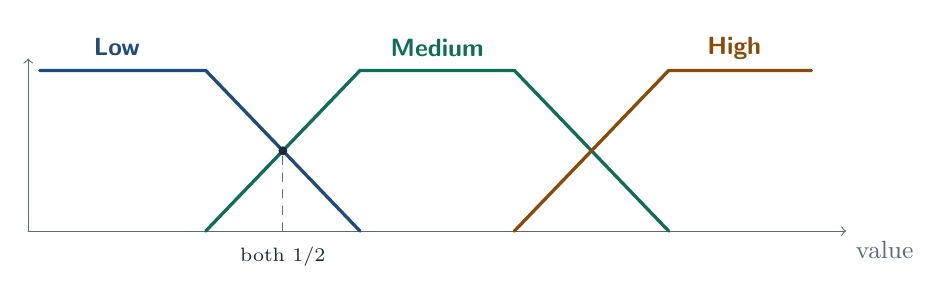
\begin{tikzpicture}[x=0.98cm, y=1.02cm, line cap=round]
  \draw[ebdmuted, ->] (0,0) -- (10.6,0) node[below right, font=\small] {value};
  \draw[ebdmuted, ->] (0,0) -- (0,2.15);
  \draw[ebblue, very thick] (0.15,2) -- (2.3,2) -- (4.3,0);
  \node[ebblue, font=\sffamily\small\bfseries, anchor=south] at (1.15,2.06) {Low};
  \draw[ebdgreen, very thick] (2.3,0) -- (4.3,2) -- (6.3,2) -- (8.3,0);
  \node[ebdgreen, font=\sffamily\small\bfseries] at (5.3,2.28) {Medium};
  \draw[ebamber, very thick] (6.3,0) -- (8.3,2) -- (10.15,2);
  \node[ebamber, font=\sffamily\small\bfseries] at (9.15,2.28) {High};
  \draw[dashed, ebdmuted] (3.3,0) -- (3.3,1.0);
  \fill[ebdink] (3.3,1.0) circle (1.6pt);
  \node[ebdink, font=\scriptsize, anchor=north] at (3.3,-0.08) {both \(1/2\)};
\end{tikzpicture}
\caption{A sketch of three overlapping labels. The search places the real boundaries on each numeric column, so ``Medium age'' means the middle band of \emph{this} table. A person near a boundary matches two labels at once. Categories such as sex match at 1 or at 0.}
\end{figure}

\noindent
These notebooks ask for three words on each numeric column (\fn{n\_linguistic\_variables=3}) and for Type-1 sets (\fn{FUZZY\_SETS.t1}), so each match is a single number in \([0,1]\). The library can also build Type-2 sets, which put a band of uncertainty around the match. The demos do not. Categories such as sex, port, or anaemia stay categories: a condition reads ``Sex is female'' or ``anaemia is 0'', with a match of 1 or 0.

\subsection{How a sentence fires}

When a rule has several conditions, the matches are multiplied. That product is the firing strength. If sex matches at 1 and age matches at one half, the rule fires at one half. If any condition matches at 0, the rule does not fire.

\[
\text{firing} = \mu_1 \times \mu_2 \times \cdots
\]

A rule may use at most three conditions in these demos (\fn{nAnts=3}). A condition slot can be left unused, which is why a printed rule is often shorter than three. The decision score is the firing multiplied by the rule weight. Demos 9 and 10 set \fn{ds\_mode=1}, which forces every weight to 1, so the firing alone is the score. Demo 11 sets \fn{ds\_mode=2}: the search also chooses a weight for each rule, and a modest firing can win when the weight is high.

\subsection{The winning rule}

For each person the model scores every rule. The rule with the highest score wins, and its \textbf{then} clause is the prediction. \fn{explainable\_predict} returns that prediction together with the index of the winning rule. \fn{winning\_rules\_by\_group} counts those indexes inside each sensitive group.

\begin{figure}[H]
\centering
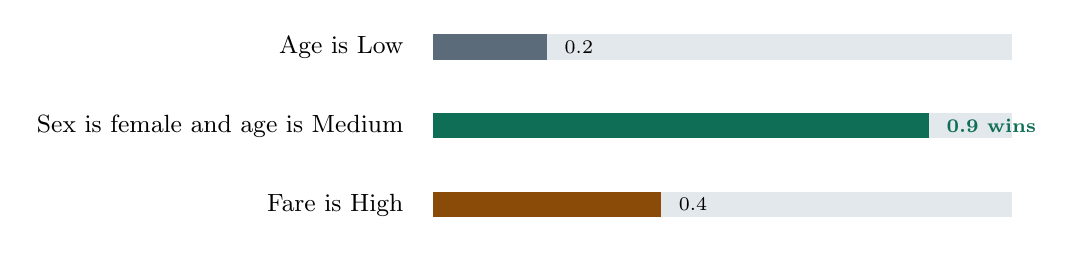
\begin{tikzpicture}[x=1cm, y=1cm]
  \node[font=\small, anchor=east] at (0,2.15) {Age is Low};
  \node[font=\small, anchor=east] at (0,1.15) {Sex is female and age is Medium};
  \node[font=\small, anchor=east] at (0,0.15) {Fare is High};
  \fill[ebdtrack] (0.25,2.0) rectangle (7.6,2.32);
  \fill[ebdtrack] (0.25,1.0) rectangle (7.6,1.32);
  \fill[ebdtrack] (0.25,0.0) rectangle (7.6,0.32);
  \fill[ebdmuted] (0.25,2.0) rectangle (1.7,2.32);
  \fill[ebdgreen] (0.25,1.0) rectangle (6.55,1.32);
  \fill[ebamber] (0.25,0.0) rectangle (3.15,0.32);
  \node[font=\scriptsize, anchor=west] at (1.8,2.16) {0.2};
  \node[font=\scriptsize\bfseries, anchor=west, ebdgreen] at (6.65,1.16) {0.9 wins};
  \node[font=\scriptsize, anchor=west] at (3.25,0.16) {0.4};
\end{tikzpicture}
\caption{The middle rule matches this person most strongly, so the model predicts that rule's outcome. With every weight equal to 1, the firing alone decides the winner.}
\end{figure}

Some fuzzy classifiers add up every rule that votes for a class and compare those totals. These notebooks keep a single winner. \fn{predict} returns that rule's consequent, and \fn{explainable\_predict} names the same rule. The sentence you read is the sentence that decided.

Beside each printed rule are three numbers.

\begin{itemize}
  \item \textbf{DS}, the dominance score, is how broadly the rule fires on its own outcome, combined with how little it fires on the other outcome. A large DS is a rule the model actually uses. A DS near zero is a rare rule.
  \item \textbf{ACC} is the share of cases in which this rule won \emph{and} was right. A rare rule can have ACC of 100\% and still barely affect anyone.
  \item \textbf{WGHT} is the weight used at decision time. It is 1.0 throughout demos 9 and 10.
\end{itemize}

\subsection{How the search chooses the sentences}
\label{sec:search}

The sentences are not written by hand in these notebooks. A genetic search keeps a population of candidate rule lists. Each candidate chooses conditions, words, and a consequent for every rule, and the search may also move the boundaries of Low, Medium, and High. In demo 11 it chooses a weight per rule as well. Each generation scores the candidates and builds the next generation from the better ones. The score, unless a notebook replaces it, is the Matthews correlation coefficient (MCC) on the training rows. MCC is positive when the predictions and the labels agree, zero when the predictions carry no information about the labels, and negative when they disagree. Its range is \(-1\) to \(+1\).

\[
\mathrm{MCC}
=
\frac{TP \cdot TN - FP \cdot FN}
{\sqrt{(TP+FP)\,(TP+FN)\,(TN+FP)\,(TN+FN)}}
\]

\(TP\) and \(TN\) are correct predictions of the event and of the other outcome. \(FP\) and \(FN\) are the two kinds of mistake.

MCC is used because accuracy flatters a lazy rule on an uneven table. On the Titanic test passengers, predicting that everyone died would be right for 136 of 235 people, about \pct{58}. The fitted rules are right for 153 of 235, about \pct{65}, and their MCC is only 0.26. On the loan test applications, approving everyone would be right for 112 of 159 people, about \pct{70}. The baseline rules are right for 94 of 159, about \pct{59}, while their MCC stays positive at 0.17 because some of the denials are correct. Accuracy went down. The correlation did not disappear. The search follows the correlation.

\begin{careful}
\textbf{The search in these notebooks is a classroom budget.} Each fit tries 12 candidate rule sets for at most 6 generations and stops after 3 generations without improvement (\fn{n\_gen=6}, \fn{pop\_size=12}, \fn{patience=3}). The library defaults are much larger. Read the stored rules as a demonstration of the measurements. A longer search can write different sentences. The way you read a printed rule stays the same.
\end{careful}

Up to 8 rules are available on the Titanic and the loans (\fn{nRules=8}), and up to 6 on heart failure. Empty slots are dropped, which is why the Titanic printout contains six rules rather than eight. The printed ``consequent'' is the 0/1 code of the outcome.

% ---------------------------------------------------------------------
\section{The three bias demos}
\label{sec:picture}

With that classifier in hand, the notebooks ask which group the sentences pick. Every number below is the run stored in the notebooks: the same train--test split (\fn{test\_size=0.33}, \fn{random\_state=42}) and the short search in Section~\ref{sec:search}.

\begin{lesson}
\textbf{Titanic (demo 9).} In the prepared table, 195 of 259 women survive and 93 of 453 men survive. On the held-out passengers the rules predict survival for 49 of 86 women and for none of 149 men.

\textbf{Heart failure (demo 10).} Death is almost equally common: 34 of 105 women and 62 of 194 men. The rules that carry the model talk about blood tests. The one rule that names sex barely fires.

\textbf{Loans (demo 11).} Approval differs by about eight percentage points in the table. The baseline rules open a gap of about thirty points on the test set. Reweighing the training rows reverses the gap. A penalty on the gap pulls the rates together and approves fewer people.
\end{lesson}

Each notebook walks through the same four questions.

\begin{enumerate}
  \item \textbf{Before any model,} how often does the event already happen in each group?
  \item \textbf{What sentences} did the search keep, and does a sentence name the sensitive column?
  \item \textbf{After the model decides,} how often is the event predicted in each group, and how often is that prediction right?
  \item \textbf{Which sentence won} for the people in each group?
\end{enumerate}

Demo 11 adds a fifth question: if we change the score the search is trying to raise, do the answers to questions 3 and 4 move?

\begin{idea}
\textbf{Two different gaps.} The gap in the labels is a property of the table. The gap in the predictions is a property of the rules. They can be large together, as on the Titanic. They can also come apart: the heart-failure labels almost agree, and the loan labels disagree only modestly, while the fitted rules disagree more.
\end{idea}

The sensitive column stays available to the rules in all three fits. On the Titanic and in the loan file it is a column the model may use. The heart-failure file uses the same pattern with \fn{sex} coded numerically: 0 is female and 1 is male.

\begin{table}[H]
\centering
\small
\begin{tabularx}{\textwidth}{@{}l Y c c@{}}
\toprule
Demo & Event being counted & Sensitive column & Rows kept \\
\midrule
9 Titanic & Survived, coded 1 & \fn{Sex} & 712 of 891 \\
10 Heart failure & Death during follow-up, coded 1 & \fn{sex} (0 woman, 1 man) & 299 of 299 \\
11 Loans & Loan approved, coded 1 & \fn{Gender} & 480 of 614 \\
\bottomrule
\end{tabularx}
\end{table}

\noindent
Incomplete Titanic rows are those missing age or the embarkation port, about one passenger in five. Incomplete loan applications are dropped the same way, and \fn{Y}/\fn{N} is recoded to 1/0. The rates below describe the rows that remain.

The event is whatever the notebook passes as \fn{positive\_label=1}. The tools do not know whether that event is a benefit. Survival and approval are benefits. Death is the clinical event, so a higher heart-failure rate is a worse outcome. The word ``positive'' in the printed tables means ``this is the event we chose to count.''

% ---------------------------------------------------------------------
\section{How a gap is measured}
\label{sec:measure}

Use the Titanic test women as the running example: 86 women, of whom 64 survived and 22 died. The rules predict survival for 49 of them. Of those 49, 33 had survived and 16 had died.

\begin{idea}
\textbf{Outcome rate} --- before the model. Among people in the group, how often did the event happen?

\[
\frac{\text{women who survived}}{\text{women}} = \frac{195}{259} \approx \pct{75}
\quad\text{in the whole prepared table.}
\]

\textbf{Selection rate} --- after the model. Among people in the group, how often is the event \emph{predicted}?

\[
\frac{49}{86} \approx \pct{57}
\quad\text{of test women are predicted to survive.}
\]

The call for the first is \fn{outcome\_rates\_by\_group}. The call for the second, together with the error rates below, is \fn{fairness\_report}.
\end{idea}

\subsection{When the prediction is wrong}

Split the group by what truly happened.

\begin{itemize}
  \item \textbf{True positive rate (TPR).} Of the people who \emph{did} experience the event, how many are predicted to experience it? For the test women, 33 of 64 survivors, about \pct{52}.
  \item \textbf{False positive rate (FPR).} Of the people who did \emph{not} experience the event, how many are predicted to experience it anyway? For the test women, 16 of 22 who died, about \pct{73}.
  \item \textbf{False negative rate} is the rest of the first group: 31 of 64 survivors are missed.
  \item \textbf{True negative rate} is the rest of the second group: 6 of 22 women who died are predicted to have died.
\end{itemize}

TPR and FPR answer a different question from the selection rate. Two groups can be selected equally often while the errors fall on different people. Two groups can also have similar error rates and very different selection rates, because the event itself was already more common in one group.

\subsection{Demographic parity and equalized odds}

Demographic parity compares selection rates. The notebook prints two summaries.

\[
\begin{aligned}
\text{difference} &= \text{highest selection rate} - \text{lowest selection rate} \\
\text{ratio} &= \text{lowest selection rate} \;/\; \text{highest selection rate}
\end{aligned}
\]

A difference of 0 and a ratio of 1 mean the groups are selected equally often. The Titanic test difference is \(49/86 - 0/149 \approx 0.57\). That printed \fn{0.57} is \textbf{57 percentage points}, the gap between \pct{57} and \pct{0}. It is the proportion \(0.57\), which is easy to misread as ``0.57 percent.''

Equalized odds compares the error rates. The printed difference is the \emph{larger} of the TPR gap and the FPR gap. On the Titanic test set the FPR gap is the larger one: women who died are predicted to survive \pct{73} of the time, and men who died are predicted to survive \pct{0} of the time.

\begin{careful}
\textbf{A ratio of 0 usually means one rate is zero.} The heart-failure test set has a false-positive rate of 0 for men, so \fn{equalized\_odds\_ratio} prints as 0 even though the TPR gap is 10 points and the FPR gap is 5 points. Read \fn{tpr\_difference} and \fn{fpr\_difference} before reading the ratio. The difference is the quantity the loan penalty uses.
\end{careful}

% ---------------------------------------------------------------------
\section{Titanic: the imbalance is already in the labels}
\label{sec:titanic}

The table records passengers and whether they survived. The prepared columns are passenger class, sex, age, siblings or spouses aboard (\fn{SibSp}), parents or children aboard (\fn{Parch}), fare, and the embarkation port. \fn{C} in a rule means Cherbourg.

\begin{table}[H]
\centering
\begin{tabular}{@{}l c r@{}}
\toprule
 & Share who survived & Count \\
\midrule
Women & \track{0.753}{ebdwomen} & 195 of 259 \\
Men   & \track{0.205}{ebdmen} & 93 of 453 \\
\bottomrule
\end{tabular}
\end{table}

\noindent
This is the state of the table before training. A rule that is allowed to say ``sex is female'' has a large, real association to copy. The historical pattern in these data, women surviving much more often than men, is visible without a model.

\subsection{The six sentences the short search kept}

Consequent 1 is survival. Consequent 0 is death. Dominance scores are rounded; the two tiniest death rules are below 0.001.

\begin{table}[H]
\centering
\small
\begin{tabularx}{\textwidth}{@{}l Y c c@{}}
\toprule
Then & Conditions & DS & Right when it wins \\
\midrule
\rowcolor{ebdrow}
Survived & Sex is female, and age is Medium & 0.11 & \pct{83} \\
Died & Age is Low, and siblings/spouses are Low & 0.04 & \pct{65} \\
Died & Sex is female, and siblings/spouses are High & 0.007 & \pct{80} \\
\rowcolor{ebdrow}
Died & Parents/children are High, and fare is Low & 0.007 & \pct{80} \\
Died & Age is Low, parents/children are Medium, fare is Medium & \(<0.001\) & \pct{79} \\
\rowcolor{ebdrow}
Died & Parents/children are Medium, fare is Low, port is Cherbourg & \(<0.001\) & \pct{50} \\
\bottomrule
\end{tabularx}
\end{table}

The survival rule is the loudest sentence in the set: its dominance score is more than twice the next rule. In ordinary words it says that a woman in the middle age band of this table survived. One quieter death rule also names sex: a woman travelling with many siblings or a spouse is predicted to have died. Naming the sensitive column is something you can see directly, which is the reason a rule model is useful in this workshop.

\subsection{What happens on the 235 held-out passengers}

The split leaves 86 women and 149 men in the test set. Of those women, 64 survived. Of those men, 35 survived.

\begin{table}[H]
\centering
\small
\begin{tabularx}{\textwidth}{@{}l Y Y@{}}
\toprule
 & Women (86) & Men (149) \\
\midrule
Truly survived & 64 & 35 \\
Predicted to survive & 49 & 0 \\
Survivors correctly predicted & 33 of 64 & 0 of 35 \\
Deaths predicted as survival & 16 of 22 & 0 of 114 \\
\bottomrule
\end{tabularx}
\end{table}

Those 49 predicted survivals are exactly the 49 women for whom the survival rule won. It wins for none of the men, so every man is predicted to have died, including the 35 men who survived. Demographic parity difference is 0.57. The larger error gap is the false-positive gap, 0.73, and that is the equalized-odds difference.

Test accuracy is 153 of 235, about \pct{65}, against \pct{58} for the rule ``everyone died.'' Test MCC is 0.26. The model has learned something, and what it has learned is concentrated on sex.

\begin{lesson}
On this table the label gap and the prediction gap point the same way. Women survive much more often, the loudest rule says that a woman in the middle age band survived, and on the test passengers that rule is the only source of predicted survivals.
\end{lesson}

% ---------------------------------------------------------------------
\section{Heart failure: similar labels, one rare rule}
\label{sec:heart}

The table has 299 patients. The event is death during follow-up. The columns are age, anaemia, creatinine phosphokinase, diabetes, ejection fraction, high blood pressure, platelets, serum creatinine, serum sodium, sex, and smoking. Ejection fraction is how much blood the heart pushes out on each beat. Serum creatinine is a blood measure related to kidney function. Serum sodium is the sodium level in the blood. Creatinine phosphokinase is an enzyme that can rise when muscle, including heart muscle, is injured. The binary flags were stored as categories, which is why a rule can say ``anaemia is 0'' (anaemia absent) and ``sex is 0'' (woman).

\begin{table}[H]
\centering
\begin{tabular}{@{}l c r@{}}
\toprule
 & Share who died & Count \\
\midrule
Women & \track{0.324}{ebdwomen} & 34 of 105 \\
Men   & \track{0.320}{ebdmen} & 62 of 194 \\
\bottomrule
\end{tabular}
\end{table}

\noindent
The two bars are the lesson in the labels. About one patient in three dies, in both groups. A model can still write a sentence that names sex. The dominance score tells you whether that sentence matters.

\begin{table}[H]
\centering
\small
\begin{tabularx}{\textwidth}{@{}l Y c c@{}}
\toprule
Then & Conditions & DS & Right when it wins \\
\midrule
\rowcolor{ebdrow}
Survived & Serum creatinine is Low & 0.54 & \pct{79} \\
Died & Ejection fraction is Low & 0.06 & \pct{82} \\
Died & Creatinine phosphokinase is Low, and platelets are Medium & 0.02 & \pct{71} \\
\rowcolor{ebdrow}
Died & Anaemia is absent, serum sodium is Medium, and sex is female & 0.006 & \pct{100} \\
\bottomrule
\end{tabularx}
\end{table}

Low serum creatinine, predicting survival, dominates the rule set. Its score is about nine times the ejection-fraction rule and about ninety times the rule that names sex. The sex rule is perfectly accurate on the few occasions it wins, and it almost never wins. Both facts are in the printout. Reading only ``the model uses sex'' would miss the score of 0.006. Reading only the label table would miss that the sentence exists.

\subsection{Predictions on the 99 test patients}

The test slice is small and a bit less even than the full table: 12 of 32 women die, and 30 of 67 men die. The fitted rules rarely predict death for anyone.

\begin{table}[H]
\centering
\small
\begin{tabularx}{\textwidth}{@{}l Y Y@{}}
\toprule
 & Women (32) & Men (67) \\
\midrule
Truly died & 12 & 30 \\
Predicted to die & 3 & 2 \\
Deaths detected & 2 of 12 & 2 of 30 \\
False alarms, among those who lived & 1 of 20 & 0 of 37 \\
\bottomrule
\end{tabularx}
\end{table}

The selection rates are about \pct{9} and \pct{3}, so the demographic-parity difference is 0.06, about six percentage points. The true-positive gap is ten points and the false-positive gap is five, so the equalized-odds difference is 0.10. The equalized-odds \emph{ratio} prints as 0 because the male false-positive rate is 0. That zero is a small count, not a deep separation: it is the difference between one false alarm and none, on 20 and 37 people.

Test accuracy is 60 of 99. Predicting that nobody dies would be right for 57 of 99. Test MCC is 0.18. This short fit is a weak classifier that mostly predicts survival, slightly more willing to predict death for a woman.

\begin{careful}
These sentences are a six-generation search on a few hundred patients. They are a way to practise reading a rule, and they agree in direction with the usual clinical reading of creatinine and ejection fraction. They are not a clinical guideline.
\end{careful}

\begin{lesson}
A label gap near zero does not promise that no rule names the sensitive column. Look at the dominance score next to any rule that does. Here the column is named by a rule the model almost never uses, and the prediction gap on the test patients is a handful of people.
\end{lesson}

% ---------------------------------------------------------------------
\section{Loans: changing the score the search maximises}
\label{sec:loans}

Each row is a loan application. The prepared columns are gender, married status, number of dependants, education, self-employment, the two incomes, the loan amount, the term, credit history, and the property area. Approval is 1 and denial is 0.

\begin{table}[H]
\centering
\begin{tabular}{@{}l c r@{}}
\toprule
 & Share approved & Count \\
\midrule
Women & \track{0.628}{ebdwomen} & 54 of 86 \\
Men   & \track{0.706}{ebdmen} & 278 of 394 \\
\bottomrule
\end{tabular}
\end{table}

\noindent
The label gap is about eight percentage points, 278/394 against 54/86. Men are also most of the table: 394 of 480 applicants. The test set then contains 22 women and 137 men. Two women moving from one side of a count to the other changes the female rate by about nine points (\(2/22\)). Read the loan percentages together with the counts.

The notebook fits the same short search three times. Gender remains a column in all three, so a rule is still allowed to say ``Gender is Male.'' What changes is the score.

\subsection{Baseline: maximise MCC}

The search sees the training rows as they are. On the 159 test applications it approves 6 of 22 women and 79 of 137 men.

\begin{table}[H]
\centering
\small
\begin{tabularx}{\textwidth}{@{}l Y Y@{}}
\toprule
Baseline test result & Women (22) & Men (137) \\
\midrule
Truly approved & 15 & 97 \\
Predicted approved & 6 & 79 \\
Approvals correctly predicted & 5 of 15 & 61 of 97 \\
Denials predicted as approval & 1 of 7 & 18 of 40 \\
\bottomrule
\end{tabularx}
\end{table}

The selection rates are about \pct{27} and \pct{58}. The demographic-parity difference is 0.30. True-positive rates are 5/15 and 61/97, a gap of about 30 points. False-positive rates are 1/7 and 18/40, a gap of about 31 points. Equalized-odds difference is the larger of those, 0.31.

Accuracy is 94 of 159, about \pct{59}, which is below the \pct{70} of ``approve everyone.'' MCC is 0.17. The rules are picking up a real but modest association, and they approve men much more often than women.

\subsection{Reweighing: make gender and the decision independent in the training weights}

Kamiran and Calders (2012) give every training row a weight that depends only on its group and its label:

\[
w(a, y)
=
\frac{P(Y = y)\; P(A = a)}{P(A = a,\; Y = y)}.
\]

\(A\) is the sensitive group and \(Y\) is the label. A group--label pair that is rarer than independence would predict gets a weight above 1 and counts more. A pair that is more common gets a weight below 1. After reweighing, group and label are independent in the \emph{weighted} training sample. \fn{reweigh\_weights} computes \(w\), and \fn{weighted\_mcc\_loss} makes the search maximise MCC with those weights. The test metrics stay unweighted: they describe the original people.

A round village makes the arithmetic obvious. One hundred applicants, 50 women and 50 men. Twenty women and forty men are approved.

\begin{table}[H]
\centering
\small
\begin{tabular}{@{}l r r r@{}}
\toprule
 & Applicants & Weight & Weighted count \\
\midrule
Women approved & 20 & \(0.60 \times 0.50 / 0.20 = 1.50\) & 30 \\
Men approved & 40 & \(0.60 \times 0.50 / 0.40 = 0.75\) & 30 \\
Women denied & 30 & \(0.40 \times 0.50 / 0.30 = 0.67\) & 20 \\
Men denied & 10 & \(0.40 \times 0.50 / 0.10 = 2.00\) & 20 \\
\bottomrule
\end{tabular}
\end{table}

\noindent
Approved women and denied men were the uncommon pairs, so they count more. In the weighted village, 30 women and 30 men are approved. The loan notebook does this with the real training rows, then asks the genetic search to find rules that score well on the weighted MCC.

In the stored run the test set moves past equality and out the other side.

\begin{table}[H]
\centering
\small
\begin{tabularx}{\textwidth}{@{}l Y Y@{}}
\toprule
Reweighed test result & Women (22) & Men (137) \\
\midrule
Predicted approved & 17 of 22 & 45 of 137 \\
Approvals correctly predicted & 12 of 15 & 37 of 97 \\
Denials predicted as approval & 5 of 7 & 8 of 40 \\
\bottomrule
\end{tabularx}
\end{table}

Women are now approved about \pct{77} of the time and men about \pct{33}. The difference is 0.44, larger than the baseline gap of 0.30, and it points the other way. Accuracy falls to 83 of 159, about \pct{52}. MCC falls only slightly, to 0.15.

\begin{idea}
Reweighing changes how much each training row counts. It does not constrain the test gap directly. With only six generations, the stored search overshoots: the test rates cross and the gap grows. A reweighing step can be checked only by reading the test table, which is what the notebook prints.
\end{idea}

\subsection{A penalty: charge the search for unequal approval rates}

The second repair replaces the score with

\[
\mathrm{score}
=
\mathrm{MCC}
-
\lambda
\times
(\text{highest selection rate} - \text{lowest selection rate}),
\]

with \(\lambda = 0.2\), the value used in the workshop and passed as \fn{lam=0.2}. The selection rates inside this formula are computed on the training rows, during the search. \fn{fairness\_regularized\_loss} builds that score.

On the scale of these demos, MCC is often between about 0.10 and 0.25. A thirty-point gap then costs \(0.2 \times 0.30 = 0.06\), a large slice of the score. The search has a concrete reason to trade some correlation for closer rates. It can spend that trade by approving fewer people in the higher group, by approving more people in the lower group, or by both.

The stored test result is the first of those, applied to both groups.

\begin{table}[H]
\centering
\small
\begin{tabularx}{\textwidth}{@{}l Y Y@{}}
\toprule
Penalised test result & Women (22) & Men (137) \\
\midrule
Predicted approved & 4 of 22 & 33 of 137 \\
Approvals correctly predicted & 3 of 15 & 26 of 97 \\
Denials predicted as approval & 1 of 7 & 7 of 40 \\
\bottomrule
\end{tabularx}
\end{table}

The rates are about \pct{18} and \pct{24}. The difference is 0.06. The true-positive gap shrinks to about seven points and the false-positive gap to about three. Accuracy is 68 of 159, about \pct{43}, and MCC is 0.10. Both groups are approved far less often than the \pct{69} approval rate of the prepared table. Equal selection rates and a generous approval policy are different goals. The printed accuracy, or the MCC, is what shows the cost.

\subsection{The three test gaps side by side}

\begin{table}[H]
\centering
\small
\begin{tabularx}{\textwidth}{@{}l Y Y c c@{}}
\toprule
Fit & Women approved & Men approved & Gap & Right \\
\midrule
Baseline MCC & 6 of 22 & 79 of 137 & 30 pts & 94/159 \\
\rowcolor{ebdrow}
Reweighed MCC & 17 of 22 & 45 of 137 & 44 pts, reversed & 83/159 \\
MCC minus \(0.2\times\)gap & 4 of 22 & 33 of 137 & 6 pts & 68/159 \\
\bottomrule
\end{tabularx}
\end{table}

\noindent
``Approve everyone'' would have been right on 112 of these 159 applications. All three fits are below that accuracy. The penalty fit is the most even and the least accurate.

\begin{lesson}
On this short run, reweighing does not land on equal test rates: it reverses the gap. The penalty does land near equal test rates, by approving 4 of 22 women and 33 of 137 men. Report the gap and the accuracy together. Demographic parity is silent about whether the shared rate is high or low.
\end{lesson}

The notebook's introduction also names a third workshop idea: drop the gender column before training. The cells that run do not do this. Dropping the column means no rule can literally say ``Gender is Male.'' Married status, income, and property area can still differ by gender, so the selection rates can still diverge. The two repairs that \emph{are} fitted leave the column in place and change only the score.

% ---------------------------------------------------------------------
\section{Reading a notebook without getting lost}
\label{sec:howto}

Open the notebook beside this guide. On Colab, run the first cell once. It clones the repository and installs it. If the next cell cannot import \fn{ebdai}, restart the runtime and run all cells again.

\begin{enumerate}
  \item \textbf{Read the outcome-rate table before the fit.} Write down the two counts. That is the label gap, and it does not depend on the genetic search.
  \item \textbf{Circle any rule that names the sensitive column.} Then read its DS. A rule with DS near zero is a sentence the model almost never uses. A rule with the largest DS is the sentence doing the work.
  \item \textbf{Read \fn{selection\_rate} as a count.} Multiply by \(n\). On these stored runs the products are whole numbers of people: 49 of 86, 0 of 149, 6 of 22, 79 of 137.
  \item \textbf{Read TPR and FPR from the same row.} Selection rate says who receives the prediction. TPR and FPR say whether that prediction is right for people who did, and did not, experience the event.
  \item \textbf{Treat a printed ratio of 0 as ``some rate is zero,''} then look at the differences. Section~\ref{sec:measure} shows why, on the heart-failure test set.
  \item \textbf{If you change the score, print accuracy beside the new gap.} The loan table in Section~\ref{sec:loans} is the pattern: one repair overshoots, and the other buys a smaller gap with a lower accuracy.
\end{enumerate}

Demos 9 and 10 are the same shape. Demo 10 is the control case, where the label rates already agree. Demo 11 repeats the baseline and then fits the two alternative scores. The bar charts are the same counts drawn as bars: outcome rate by group, and the share of each group for whom a given rule won.

The group order in a printed frame follows the code, so heart-failure fairness rows can list men (1) before women (0), while the outcome-rate table lists 0 then 1. The counts identify the groups: 32 and 67 on the heart-failure test set, 22 and 137 on the loan test set.

% ---------------------------------------------------------------------
\Needspace{8\baselineskip}
\section{Glossary and sources}
\label{sec:glossary}

\begin{table}[H]
\centering
\small
\begin{tabularx}{\textwidth}{@{}l Y@{}}
\toprule
Term in the notebook & What it means here \\
\midrule
Explainable by design & The trained model is already readable. The winning rule is the explanation. \\
\rowcolor{ebdrow}
Meaningful information about the logic & The GDPR phrase for the procedure actually applied to that person, in plain language (C-203/22). \\
High-risk AI system & An AI Act category. Credit scoring is Annex~III, from 2~December 2027. Many medical devices follow on 2~August 2028. \\
\rowcolor{ebdrow}
Membership \(\mu\) & How fully a value fits one word, from 0 to 1. \\
Firing strength & Product of the memberships in one rule. Multiplied by the rule weight to score it. \\
\rowcolor{ebdrow}
Antecedent / consequent & The IF side of a rule, and the class on the THEN side. \\
Outcome rate & Share of the group for whom the event already happened. \\
\rowcolor{ebdrow}
Selection rate & Share of the group for whom the model predicts the event. \\
TPR, FPR & Among people who did, or did not, experience the event, the share predicted to experience it. \\
\rowcolor{ebdrow}
Demographic parity & The selection rates are equal. The printed difference is highest minus lowest. \\
Equalized odds & The TPR values are equal and the FPR values are equal. The printed difference is the larger of those two gaps. \\
\rowcolor{ebdrow}
Winning rule & The rule with the highest score for that person. Its consequent is the prediction. \\
DS & How much a rule is used on its own outcome. Large means active. Near zero means rare. \\
\rowcolor{ebdrow}
ACC on a rule & When this rule won, how often it was right. \\
MCC & Correlation between predictions and labels, from \(-1\) to \(+1\), used as the search score. \\
\rowcolor{ebdrow}
\fn{ds\_mode=1} & Rule weights are all 1. The match decides the winner. Demos 9 and 10. \\
\fn{ds\_mode=2} & The search chooses a weight per rule. Demo 11. \\
\rowcolor{ebdrow}
Reweighing & Training weights \(P(Y)P(A)/P(A,Y)\), then weighted MCC. \\
Fairness penalty & Training score \(\mathrm{MCC} - 0.2 \times\) (selection-rate gap). \\
\bottomrule
\end{tabularx}
\end{table}

{\small
\Needspace{14\baselineskip}
\hyphenation{Fernandez Fumanal Idocin Kamiran Calders}
\paragraph{Notebooks.}
\begin{itemize}[itemsep=0.2em]
  \item Demo 9, Titanic labels and rules:\\
  {\footnotesize\url{https://colab.research.google.com/github/HAISymbiosis/EBD-AI/blob/main/Demos/09_bias_titanic.ipynb}}
  \item Demo 10, heart-failure death:\\
  {\footnotesize\url{https://colab.research.google.com/github/HAISymbiosis/EBD-AI/blob/main/Demos/10_bias_heart_failure.ipynb}}
  \item Demo 11, loan approval, reweighing, and the penalised score:\\
  {\footnotesize\url{https://colab.research.google.com/github/HAISymbiosis/EBD-AI/blob/main/Demos/11_bias_loan_fairness.ipynb}}
\end{itemize}

\paragraph{Where the ideas come from.}
The tables and the original workshop are WorkshopIgualdad2025 (Raquel Fernandez Peralta and Javier Fumanal Idocin). The reweighing formula is Kamiran and Calders, ``Data preprocessing techniques for classification without discrimination,'' \emph{Knowledge and Information Systems} 33 (2012). Equalized odds is the criterion in Hardt, Price, and Srebro, ``Equality of opportunity in supervised learning,'' NeurIPS 2016; \fn{ebdai} computes the gaps itself and does not call Fairlearn. MCC is Matthews, ``Comparison of the predicted and observed secondary structure of T4 phage lysozyme,'' \emph{Biochimica et Biophysica Acta} 405 (1975). The fuzzy rules, the genetic search, and the winning-rule decision are the \fn{ex\_fuzzy} classifier used by the notebooks.

\paragraph{The regulatory map.}
Regulation~(EU)~2024/1689 is the AI Act; Articles~10, 13, 14 and~86 and Annex~III, point~5(b), are the provisions used above. Regulation~(EU)~2026/1744 sets the high-risk dates at 2~December 2027 and 2~August 2028. The explanation already due for automated decisions about people is in the GDPR, Articles~13(2)(f), 14(2)(g), 15(1)(h) and~22, as read by the Court of Justice in C-203/22, \emph{CK v Dun \& Bradstreet Austria}, 27~February 2025. Equal access for women and men to goods and services, including banking, is Directive~2004/113/EC.
}

\end{document}
